%%%%%%%%%%%%%%%%%%%%%%%%%%%%%%%%%%%%%%%%%%%%%%%%%%%%%%%%%%%%%%%%%%%%%%
% LaTeX Template: Curriculum Vitae
%
% Source: http://www.howtotex.com/
% Feel free to distribute this template, but please keep the
% referal to HowToTeX.com.
% Date: July 2011
% 
%%%%%%%%%%%%%%%%%%%%%%%%%%%%%%%%%%%%%%%%%%%%%%%%%%%%%%%%%%%%%%%%%%%%%%
% How to use writeLaTeX: 
%
% You edit the source code here on the left, and the preview on the
% right shows you the result within a few seconds.
%
% Bookmark this page and share the URL with your co-authors. They can
% edit at the same time!
%
% You can upload figures, bibliographies, custom classes and
% styles using the files menu.
%
% If you're new to LaTeX, the wikibook is a great place to start:
% http://en.wikibooks.org/wiki/LaTeX
%
%%%%%%%%%%%%%%%%%%%%%%%%%%%%%%%%%%%%%%%%%%%%%%%%%%%%%%%%%%%%%%%%%%%%%%
\documentclass[paper=a4,fontsize=11pt]{scrartcl} % KOMA-article class
							
\usepackage[english]{babel}
\usepackage{wrapfig}
\usepackage[protrusion=true,expansion=true]{microtype}
\usepackage{amsmath,amsfonts,amsthm}     % Math packages
\usepackage{graphicx}                    % Enable pdflatex
\usepackage[svgnames]{xcolor}            % Colors by their 'svgnames'
\usepackage{geometry}
	\textheight=700px                    % Saving trees ;-)
\usepackage{url}

\frenchspacing              % Better looking spacings after periods
\pagestyle{empty}           % No pagenumbers/headers/footers
\definecolor{lightskyblue}{rgb}{0.53,0.81,0.98}
\definecolor{ashgrey}{rgb}{0.7, 0.75, 0.71}
%%% Custom sectioning (sectsty package)
%%% ------------------------------------------------------------


\sectionfont{%			            % Change font of \section command
	\usefont{OT1}{phv}{m}{n}%		% bch-b-n: CharterBT-Bold font
	\sectionrule{0pt}{0pt}{-5pt}{2pt}}

%%% Macros
%%% ------------------------------------------------------------
\newlength{\spacebox}
\settowidth{\spacebox}{8888888888}			% Box to align text
\newcommand{\sepspace}{\vspace*{1em}}		% Vertical space macro

\newcommand{\MyName}[1]{ % Name
		\Huge \usefont{OT1}{phv}{b}{n} \hfill #1
		\par \normalsize \normalfont}
		
\newcommand{\MySlogan}[1]{ % Slogan (optional)
		\large \usefont{OT1}{phv}{m}{n}\hfill \textit{#1}
		\par \normalsize \normalfont}

\newcommand{\NewPart}[1]{\section*{\uppercase{#1}}}

\newcommand{\PersonalEntry}[2]{
		\noindent\hangindent=2em\hangafter=0 % Indentation
		\parbox{\spacebox}{        % Box to align text
		\textit{#1}}		       % Entry name (birth, address, etc.)
		\hspace{1.5em} #2 \par}    % Entry value

\newcommand{\SkillsEntry}[2]{      % Same as \PersonalEntry
		\noindent\hangindent=2em\hangafter=0 % Indentation
		\parbox{\spacebox}{        % Box to align text
		\textit{#1}}			   % Entry name (birth, address, etc.)
		\hspace{1.5em} #2 \par}    % Entry value	
		
\newcommand{\EducationEntry}[4]{
		\noindent \textbf{#1} \hfill      % Study
		\colorbox{ashgrey}{%
			\parbox{6em}{%
			\hfill\color{Black}#2}} \par  % Duration
		\noindent \textit{#3} \par        % School
		\noindent\hangindent=2em\hangafter=0 \small #4 % Description		
		\normalsize \par}

\newcommand{\WorkEntry}[4]{				  % Same as \EducationEntry
		\noindent \textbf{#1} \hfill      % Jobname
		\colorbox{Black}{\color{White}#2} \par  % Duration
		\noindent \textit{#3} \par              % Company
		\noindent\hangindent=2em\hangafter=0 \small #4 % Description
		\normalsize \par}

%%% Begin Document
%%% ------------------------------------------------------------
\begin{document}
% you can upload a photo and include it here...
\begin{wrapfigure}{l}{0.25\textwidth}
	\vspace*{-2em}
		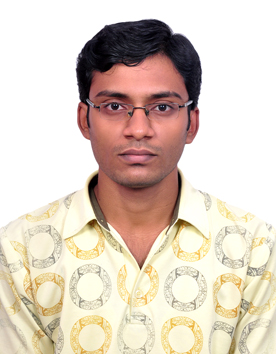
\includegraphics[width=0.15\textwidth]{10.jpg}
\end{wrapfigure}


\MyName{Naveen Cherupally}
\MySlogan{Curriculum Vitae}

\sepspace

\vspace*{5mm}
%%% Personal details
%%% ------------------------------------------------------------

\NewPart{Personal details}{}

\PersonalEntry{Birth}{October 4, 1991}
\PersonalEntry{Address}{H.No: 52, Venkateshwara nagar colony, Lothkunta, Secunderabad-15}
\PersonalEntry{Phone}{+91-8125760968}
\PersonalEntry{Mail}{\url{ncherupally@gmail.com}}

%%% Education
%%% ------------------------------------------------------------
\NewPart{Education}{}

\EducationEntry{Bachelor of Technology in Computer Engineering\\Indian Institute of Information Technology Design \& Manufacturing  \\ Kancheepuram}{2010 - 2014}{An Institute under MHRD, Govt of India}{I successfully completed my B.tech in Computer Engineering with a CGPA of \textbf{6.94} out of 10 with no backlogs(CGPA of \textbf{7.81} in the last 4 semesters). }
\renewcommand\thetable{}
\begin{table}[!ht]
\centering
    \begin{tabular}{ | c | c | c | c | c | c | c | c |}
    \hline
    1 & 2 & 3 & 4 & 5 & 6 & 7 & 8 \\ \hline
    5.68 & 6.04 & 6.26 & 6.17 & 8.2 & 6.67 & 7.6 & 8.76\\ \hline
    
    \end{tabular}
    \caption{Semester wise gpa}
    \label{Table1}
\end{table}
\sepspace

\EducationEntry{Intermediate\\Narayana Junior College, Dilsukhnagar, Hyderabad}{2007 - 2009}{Board of Intermediate Education, Andhra Pradesh}{I successfully completed my intermediate education with a percentage of \textbf{94.2}.}
\sepspace

\EducationEntry{SSC\\Bhashyam High School, R.K.puram, Hyderabad}{2006 - 2007}{Board of Secondary Education, Andhra Pradesh}{I successfully completed my class X with a percentage of \textbf{88.6}.}


\iffalse
%%% Work experience
%%% ------------------------------------------------------------
\NewPart{Work experience}{}

\EducationEntry{Job name}{2011-present}{Company Name inc., Full-time}{Job description goes here. To maintain a stylish look, try to fill this description with a few lines of text. Do the same for the other entries in this section.}
\sepspace

\EducationEntry{Job name}{2010-2011}{Company Name inc., Part-time}{Job description goes here. To maintain a stylish look, try to fill this description with a few lines of text. Do the same for the other entries in this section.}
\fi


\NewPart{Areas of Interest}{}
\begin{itemize}
\item Data structures, Design and Analysis of Algorithms
\item Operating Systems
\end{itemize}


%%% Skills
%%% ------------------------------------------------------------
\NewPart{Programming Languages known}{}


\SkillsEntry{Good Level}{C, C++}
\vspace*{3mm}
\SkillsEntry{Intermediate Level}{MySQL}
\vspace*{3mm}
\SkillsEntry{Software}{\textsc{Matlab}}


\newpage
\NewPart{Academic Strength}{}
\begin{itemize}
\item Coding in High Level Languages.
\end{itemize}


\NewPart{Major Assignments done as part of our courses in B.Tech}{}
\begin{itemize}
\item Implemented \textbf{Stop and Wait} protocol as part of my computer networks course.
\item Designed and Developed \textbf{Income Tax Calculator} as a group of four members in the team as part of our Software Engineering course.
\item We have taken care of cognitive and usability issues in \textbf{Income Tax Calculator} as part of our Human Computer Interaction course.
\end{itemize}

\NewPart{B.Tech mini-project}{}
Mini-project titled \textbf{Complexity of Steiner Tree Variants} under the guidance of Dr. Sadagopan, Department of Computer Engineering.
\NewPart{B.Tech thesis Details}{}
Thesis titled \textbf{Steiner Tree Heuristics for Split and Bipartite Graphs} under the guidance of Dr. Sadagopan, Department of Computer Engineering.
\\
%%% References
%%% ------------------------------------------------------------
\NewPart{Achievements}{}
\begin{itemize}
\item Qualified in GATE-2015 with a score of 673 and \textbf{All India Rank of 923}.
\item Won 3 gold medals for athletics(3.5 km marathon, 4x400 relay, 4x100 relay) in inter IIIT sports meet TWARAN conducted by IIITM Gwalior in 2013.
\item Won 3 silver and 1 bronze medal for athletics(100 meters, 4x100, 4x400, 3.5 km marathon) in inter IIIT sports meet TWARAN conducted by IIITM Gwalior in 2012.
\end{itemize}


\NewPart{Extra Curricular activities}{}
\begin{itemize}
\item Worked as the secretary for RUNNERS CLUB in our institute.
\item Worked as a sports coordinator in our institute. 
\item Worked as the NSS volunteer.
\item Worked as the security coordinator for SAMGATHA (cultural and technical fest) in our institute.
\end{itemize}


I do hereby declare that what is stated above is true to the best of my knowledge.
\vspace*{7mm}
\newline
Naveen C
\newline
\today
\end{document}
